% 
% Annual Cognitive Science Conference
% Sample LaTeX Paper -- Proceedings Format
% 

% Original : Ashwin Ram (ashwin@cc.gatech.edu)       04/01/1994
% Modified : Johanna Moore (jmoore@cs.pitt.edu)      03/17/1995
% Modified : David Noelle (noelle@ucsd.edu)          03/15/1996
% Modified : Pat Langley (langley@cs.stanford.edu)   01/26/1997
% Latex2e corrections by Ramin Charles Nakisa        01/28/1997 
% Modified : Tina Eliassi-Rad (eliassi@cs.wisc.edu)  01/31/1998
% Modified : Trisha Yannuzzi (trisha@ircs.upenn.edu) 12/28/1999 (in process)
% Modified : Mary Ellen Foster (M.E.Foster@ed.ac.uk) 12/11/2000
% Modified : Ken Forbus                              01/23/2004
% Modified : Eli M. Silk (esilk@pitt.edu)            05/24/2005
% Modified : Niels Taatgen (taatgen@cmu.edu)         10/24/2006
% Modified : David Noelle (dnoelle@ucmerced.edu)     11/19/2014
% Modified : Roger Levy (rplevy@mit.edu)     12/31/2018



%% Change "letterpaper" in the following line to "a4paper" if you must.

\documentclass[10pt,letterpaper]{article}

\usepackage{cogsci}

\cogscifinalcopy % Uncomment this line for the final submission 

\usepackage{graphicx} %for figures
\usepackage{pslatex}
\usepackage[natbibapa]{apacite}
\usepackage{float} % Roger Levy added this and changed figure/table
                   % placement to [H] for conformity to Word template,
                   % though floating tables and figures to top is
                   % still generally recommended!

%\usepackage[none]{hyphenat} % Sometimes it can be useful to turn off
%hyphenation for purposes such as spell checking of the resulting
%PDF.  Uncomment this block to turn off hyphenation.


%\setlength\titlebox{4.5cm}
% You can expand the titlebox if you need extra space
% to show all the authors. Please do not make the titlebox
% smaller than 4.5cm (the original size).
%%If you do, we reserve the right to require you to change it back in
%%the camera-ready version, which could interfere with the timely
%%appearance of your paper in the Proceedings.

%\title{[working title] Calling it what it is: Novel categories are distinct from Not-categories}

\title{Novel categories are distinct from ``Not''-categories}
 
\author{{\large \bf Shi Xian Liew (liew2@wisc.edu)} \\
  Department of Psychology, 1202 W. Johnson Street \\
  Madison, WI 53706 USA
  \AND {\large \bf Joseph L. Austerweil (austerweil@wisc.edu)} \\
  Department of Psychology, 1202 W. Johnson Street \\
  Madison, WI 53706 USA}


\begin{document}

\maketitle


\begin{abstract}

  The categorization literature often considers two types of categories as equivalent: (a) standard categories and (b)
  negation categories. For example, category learning studies typically conflate learning categories A and B with
  learning categories A and NOT A. This study represents the first attempt at delineating these two separate types of
  generated categories. We specifically test for differences in the distributional structure of generated categories,
  demonstrating that categories identified as \emph{not} what was known are larger and wider-spread compared to
  categories that were identified with a specific label. We also observe consistency in distributional structure across
  multiple generated categories, replicating and extending previous findings. These results are discussed in the context
  of providing a foundation for future modeling work.

\textbf{Keywords:} 
categorization; category generation; contrast; category learning; 
\end{abstract}


\section{Introduction}
% Within the broader field of categorization, the study of category generation has
% been gaining traction in recent decades. This specific topic is primarily
% concerned with
%People are remarkable in their capacity to innovate new and different ideas. Is creating a new idea the same as creating a different idea? Consider a jazz musician who wants to generate music in a new genre. Is that the same as wanting to generate music that is {\em not} jazz? Both new categories of music are distinct from jazz. The former is identified as its own category and the latter is identified in relation to a known category.

People are remarkable in their capacity to innovate new and different ideas. Is creating a new idea the same as creating
a different idea? Consider a restaurant that serves one meal per night. Their chef cooked red curry last night and wants
to create and cook a new dish tonight. Is that the same as wanting to create and cook a new dish that is {\em not} red
curry? While the former is identified as its own category, the latter is identified in relation to a known category.


While categorization researchers have primarily focused their effort on classification (associating an exemplar with a
category given its features), and inference (predicting exemplar features given its category), work on category
generation -- predicting all exemplar features for a novel category -- is relatively scarce. This is surprising because
category generation is not an uncommon phenomenon -- people are constantly challenged to generate novel categories, such
as a new meal plan for the week, a new music playlist for an upcoming road trip, or a new exercise regimen to stay
healthy.

Recent category generation work has established a few key
findings. Earlier studies have shown that generated
categories tend to share distributional statistics with learned categories \citep{ward1994structured,jern2013probabilistic,thomas98}. More recently, 
\cite{austerweil2018catgen} and \cite{conaway2017packer} have found that category contrast is an important factor in category generation and learning -- computational models sensitive to the
differences between categories were a better fit to generated categories than models
which did not take categories contrast into account.

Although previous work has established a few key findings, the basic phenomena and processes involved in category
generation are still not well understood. In this article, we examine whether given a known category in a domain,
generating a new category is different from generating a category that is not the learned category. If the only category
is A, most formal accounts of categorization would consider generating a new category B as equivalent to generating not
A. In order to better understand the nature of generated categories, it is necessary to distinguish between these two
possible types of generated categories: one driven by its own identity -- an \emph{independently identified category},
and another driven by  a motivation to be not what is known -- a
\emph{category-by-negation}.

Current models of category generation do not explicitly make this distinction. One of the first computational models of category generation, \cite{jern2013probabilistic}'s hierarchical sampling model, is a Bayesian model that reproduces distributionally similar categories by assuming that the covariance matrix of features of exemplars from generated categories is generated by the same prior that generated the covariance matrix of the known categories. An alternative proposed model, PACKER \citep{conaway2017packer}, is an extension of the classic Generalized Context Model \citep[GCM;][]{nosofsky1984choice,nosofsky1986attention}. It explicitly incorporates contrast into the similarity function by including a penalty for being similar to exemplars from a known category. A contrast parameter allows candidate categories that are more different from the known category to be weighted more heavily than candidate categories similar to the known category. Both models are flexible enough to describe how generated categories can be distributionally similar (or different) from an experimenter-defined category. However, they do not distinguish between  generating an independently identified category and a category-by-negation because there is no mechanism to account for these different identities. 

This issue also extends to the methodology applied in category generation (as well as most categorization studies.) In
\cite{ward1994structured}, participants were told to generate aliens that belonged to a different species from a prior
group of aliens, without applying any specific label to this new group of aliens. Similarly,
\cite{jern2013probabilistic} instructed participants to generate a new, different type of crystal after having observed
two different types of crystals. In contrast, \cite{conaway2017packer} prompted participants to generate exemplars from
a novel ``Beta'' category, while avoiding an explicit instruction for participants to create something ``different''. In
each of these studies there appears to be an implicit assumption that generating an independently identified category is equivalent to generating a category-by-negation.

In this paper, we challenge this null assumption by positing that the explicit association of categories-by-negation to its known counterpart (i.e., the explicit identification of the to-be-generated category as \emph{not} a known category) should result in the observer taking advantage of the entire area of the feature space not occupied by the known category. In contrast, observers generating independently identified categories should be less focused on the unoccupied feature space and instead construct their categories based on the structure of known categories. From this we can predict that categories-by-negation should occupy larger areas of the feature space compared to independently identified categories. In addition, the similarity in distributional statistics should extend not only from the learned category to the first independently identified category to be generated (as previous studies have found), but also between subsequent independently identified categories. We test these predictions by adapting and extending a category generation experiment by \cite{conaway2017packer} and explore the implications of its results.


\section{Experiment}
%JLA: If possible it would be good to cite CA2017 as much as we can rather than the manuscript. It's supposed to be double blind and citing a particular manuscript in preparation all the time may cue reviewers to the identity of the authors...
Our current experiment closely mirrors the the experimental design of \cite{conaway2017packer}, where participants are first trained on a category named `Alpha' before being tasked to generate exemplars from a new category. While \cite{conaway2017packer} were primarily interested in the measuring the location of generated categories relative to learned categories, our current investigation focuses on analyzing the differences in distributional statistics across different generated categories. Consequently, in addition to varying the shape and location of the Alpha category (i.e., across different Alpha conditions where the position of the Alpha exemplars are systematically varied) in three distinct ways, we include an additional independent variable comprising three different generation conditions: a Not-Alpha condition, where participants generate a new category that is not the learned Alpha category; a Beta-Only condition, where participants generate a new category named `Beta'; and a Beta-and-Gamma condition, where participants generate a category `Beta' as well as a category `Gamma'. The resulting 3-by-3 design is applied in a between-subjects fashion -- participants can be in only one of the nine unique conditions. 

The main advantage of adapting the experiment by \cite{conaway2017packer} is that the simplicity of their stimuli allow for a straightforward test of the distributional similarities across known and generated categories. In addition, the variety of Alpha categories used (i.e., the different shapes of the Alpha categories) also allows us to observe the effect of generated category identity across multiple scenarios. 

In line with our earlier predictions, we expect that the Not-Alpha conditions on average generate categories that are larger in area and more widely dispersed than categories from the Beta-Only as well as Beta-and-Gamma conditions. In addition, we predict that within the Beta-and-Gamma conditions, the generated Beta and generated Gamma categories should be distributionally similar. 

% No interaction effects between the factors (i.e., Alpha $\times$ Generation conditions) are expected.

\subsection{Method}

\subsubsection{Participants and materials}

We recruited 240 participants through Amazon Mechanical Turk and randomly
assigned them to one of the nine unique conditions. Sample sizes of each
condition are presented in Table \ref{table:samplesize}.

Stimuli were squares that varied along two dimensions: color (grayscale
9.8\% -- 90.2\%) and size (3.0 -- 5.8cm on each side). The assignment of perceptual
features (color, size) to axes of the domain space (x, y), as well as the
direction of variation along each axis (e.g., increasing or decreasing size) was
counterbalanced across participants. Feature values were evenly-spaced on a
50-by-50 grid, giving a near-continuous space from which exemplars can be generated. An example of the feature space is presented in Figure \ref{fig:alphas}a. 

The three Alpha conditions are Cluster, Row, and Diagonal. In the Cluster condition, Alpha exemplars occupy a small area towards one corner of the feature space. In the Row condition, the exemplars are nearly equal along one feature, while equally spread out along the other feature. The Diagonal condition has Alpha exemplars equally spaced along the diagonal of the feature space in a similar fashion to the diagonal conditions of \cite{jern2013probabilistic}. In order to ensure that exemplars are not completely identical along any one feature, exemplar feature values are slightly jittered. The exact same amount of jitter is applied to all Alpha exemplars within a given Alpha condition. The locations of these different Alpha categories in the feature space are presented in Figures \ref{fig:alphas}b to \ref{fig:alphas}d.

\begin{figure}%[H]
\begin{center}
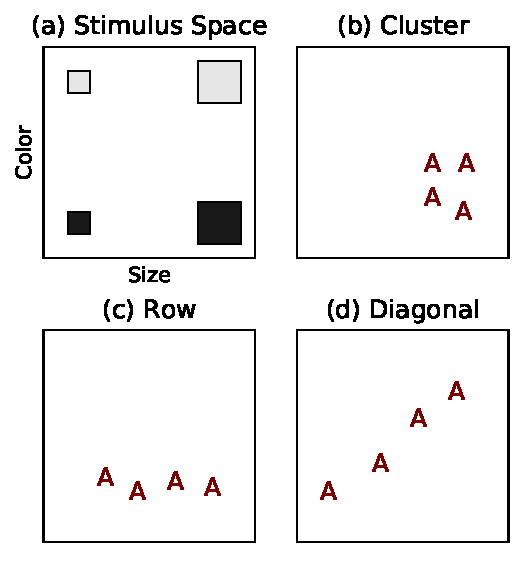
\includegraphics[width=.5\textwidth]{Figures/conditions.pdf}
\end{center}
\caption{(a) Example of stimuli located at the corners of the feature space. (b-d) Locations of Alpha category exemplars for each Alpha condition.} 
\label{fig:alphas}
\end{figure}


\subsubsection{Procedure}
In the first phase of the experiment (Figure \ref{fig:screens_learn}), participants learned the Alpha category exemplars
by observing a unique exemplar on each trial. This was repeated over a total of three blocks (four trials per block --
one corresponding to each unique exemplar,) with the order of exemplar presentation randomized within each block. Prior
to the presentation of each exemplar, a fixation cross was shown for 1000 ms. Participants were allowed to spend as much
time as they wanted on each trial and were also shown the full range of possible feature values prior to training.

\begin{figure*}%[H]
\begin{center}
    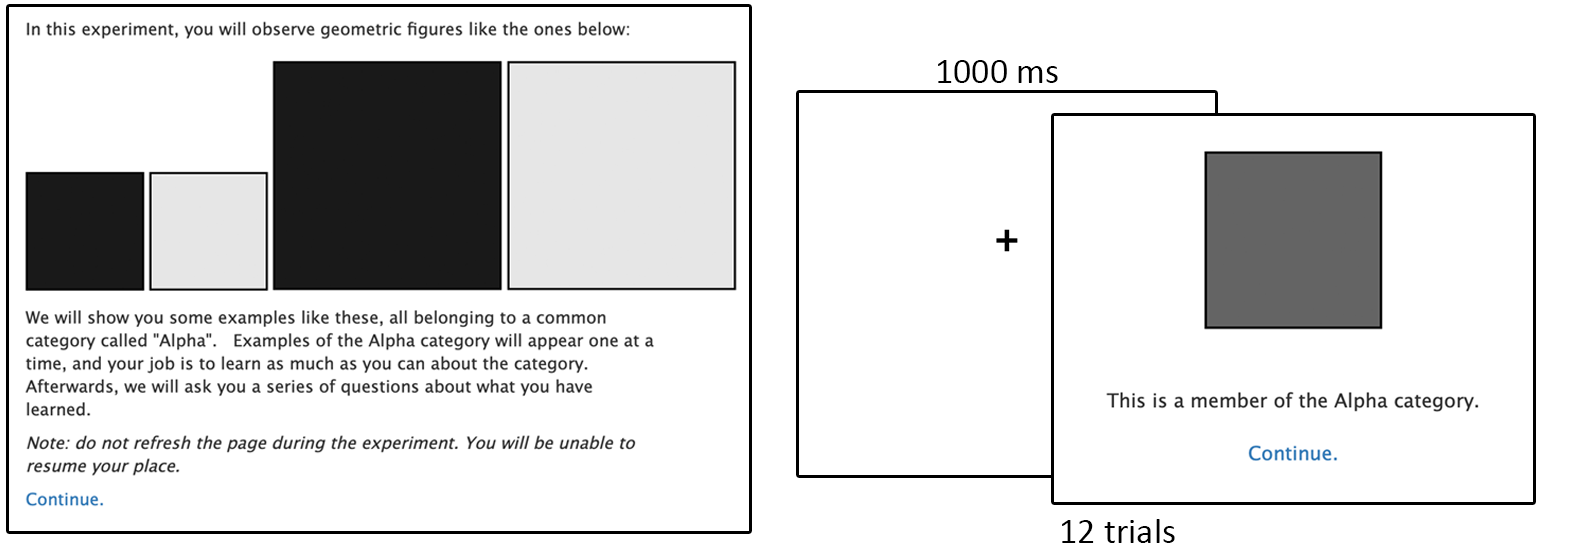
\includegraphics[width=\textwidth]{Figures/screens_learn.png}
\end{center}
\caption{Instructions and trials observed by each participant during the category learning phase. The instructions screen is
shown once, followed by 12 presentations of Alpha exemplars (4 exemplars across 3 blocks.)}
\label{fig:screens_learn}
\end{figure*}

The next phase comprised a series of generation trials (Figure \ref{fig:screens_gen}). Depending on their generation
condition, participants generated either eight exemplars from a category that was `Not-Alpha' (Not-Alpha generation
condition), eight exemplars from a category called `Beta' (Beta-Only generation condition), or four exemplars from a
category `Beta' \emph{and} four exemplars from a third category `Gamma' (Beta-and-Gamma generation condition). More
specifically, participants in the Not-Alpha generation condition were asked to produce ``what [they] think is likely to
NOT be in the Alpha category'', while participants in the other conditions were asked to produce ``what [they] think is
likely to be in the Beta [or Gamma] category''. Exemplars were generated on each trial using two on-screen sliding
scales, with each scale controlling the individual features (color and size) of the generated exemplar. Feature values
could take any one of 50 evenly-spaced values between the specified boundaries. Previously generated exemplars were not
allowed to be generated a second time. Participants were shown an on-screen preview of their exemplar on each trial as
they interacted with the sliders, but could not see previously generated exemplars or exemplars from the Alpha category.

\begin{figure*}%[H]
\begin{center}
    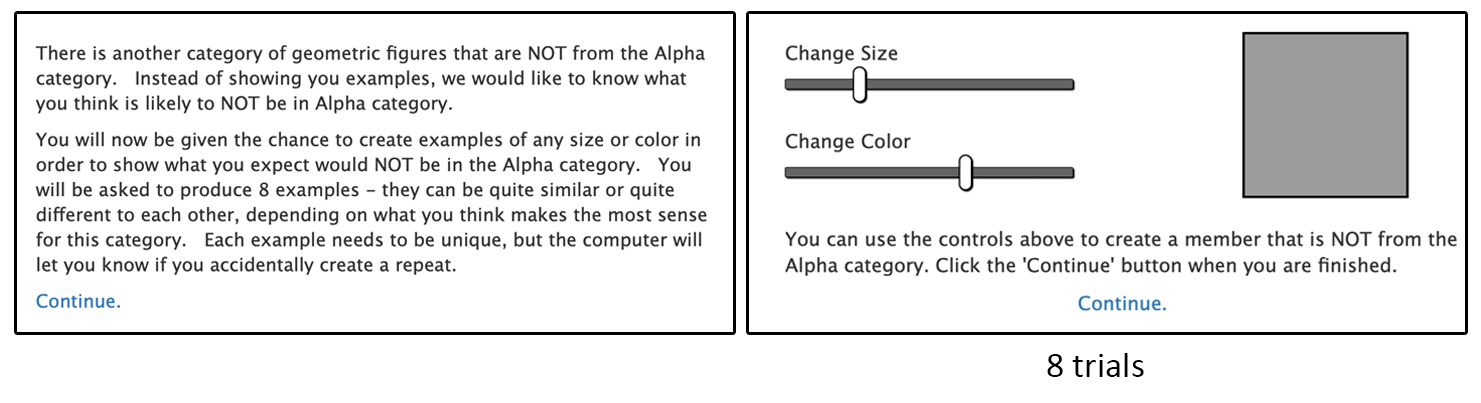
\includegraphics[width=\textwidth]{Figures/screens_gen.png}
\end{center}
\caption{Instructions and trials during the generation phase, observed by a participant in the Not-Alpha condition.
  Participants in the Beta-Only and Beta-Gamma conditions experienced similar trials, with the exception that those in
  the Beta-Gamma condition were asked to generate 4 Beta exemplars then 4 Gamma exemplars.}
\label{fig:screens_gen}
\end{figure*}

% \begin{figure*}%[H]
% \begin{center}
%     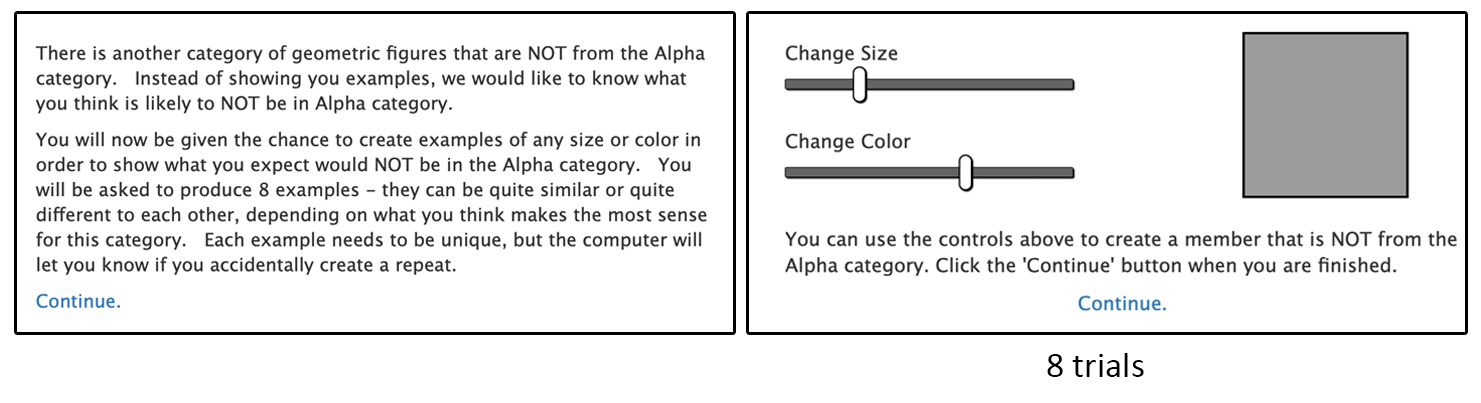
\includegraphics[width=\textwidth]{Figures/screens_gen.png}
% \end{center}
% \caption{Experimental trials observed by a participant in the Not-Alpha condition. Participants in the Beta-Only and
%   Beta-Gamma conditions experienced similar trials, with the exception that those in the Beta-Gamma condition were asked
%   to generate 4 Beta exemplars then 4 Gamma exemplars.}
% \label{fig:profile}
% \end{figure*}

\begin{table}[H]
\begin{center} 
\caption{Sample sizes for each condition.} 
\label{table:samplesize} 
\vskip 0.12in
\begin{tabular}{llll} 
\hline
Generation Condition    &  Cluster & Row & Diagonal \\
\hline
Not-Alpha      &   26 & 28 & 25 \\
Only Beta      &   30 & 27 & 25 \\
Beta-and-Gamma &   26 & 27 & 26 \\
\hline
\end{tabular} 
\end{center} 
\end{table}

\subsubsection{Analyses}

We analyze our data in two stages. First, to provide a coarse overview of the distribution of different patterns of
generated categories, we classify the generated categories into six different profiles: Positives, where the correlation
between the dimensions is more than $r$; Negatives, where the correlation between the dimensions is less than $-r$;
Rows, where the range of values across the x dimension is at least $d$ times more than the range across the y dimension;
Columns, where the range of y dimension values is at least $d$ times more than the range of x dimension values;
Clusters, where the ranges across both dimensions are less than $a$; and Dispersed, where the ranges across both
dimensions are more than $a$. Next, we compare the generated categories on four key distributional measures: ranges of
each feature, the feature correlations, and the area enclosed by the generated exemplars in the feature space (i.e.,
their convex hull). Differences along each of these statistics are performed using Bayesian $t$-tests
\citep{rouder2009bayesian}, yielding Bayes factors ($BF_{01}$) which indicate evidence for the null hypothesis when
$BF_{01} > 1$, with larger values indicating greater evidence for the null hypothesis. $BF_{01} < 1$ indicates evidence
for the alternative hypothesis. Interpretations of the sizes of Bayes factors are guided by \cite{jeffreys1961}.

\subsection{Results}

We took a subset of the data and tuned each of the profiling parameters such that the profiles of this subset were
adequately captured. Subsequently, we applied this profiling scheme to the entire dataset. Overall, we found that
setting $r = .7$, $a = .25$, and $d = 5$ was useful in capturing the different profiles of generated categories. The
results were robust to moderate variations in the profiling parameters (e.g., setting $.5 < r < .9$, $.1 < a < .4$, and
$ d > 1 $ returned very similar results.) A representative sample of each profile is shown in Figure \ref{fig:samples}
and the frequency plot of the different profiles is presented in Figure \ref{fig:profile}.

The most striking patterns to note here are the high frequencies of Row category profiles from participants in the Row conditions, and the high frequencies of Dispersed category profiles from participants in the Not-Alpha conditions. The former indicates that the distributional similarities between learned and generated categories are especially strong in the Row conditions, while the latter provides preliminary evidence that generated categories from the Not-Alpha conditions tends to be more widely dispersed. Also noteworthy are the low counts of both Positive and Negative category profiles across the whole data set -- in contrast to the Row conditions, this indicates low similarity in distributional structure between the learned and generated categories for the Diagonal condition.

%Note that the trained category exemplars (labeled as A in the figure) 

\begin{figure}[H]
\begin{center}
    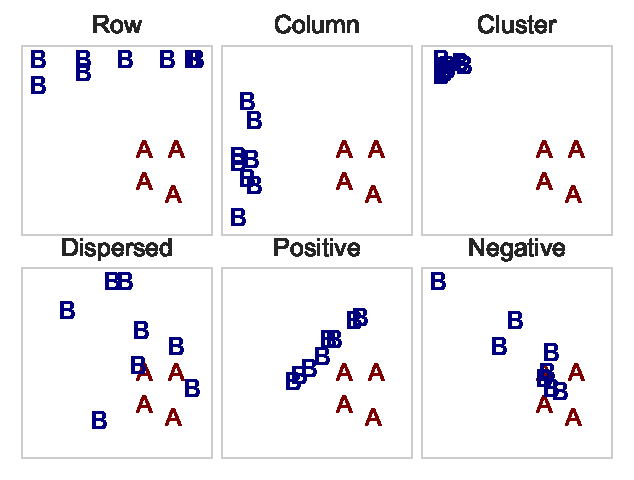
\includegraphics[width=.5\textwidth]{Figures/samples.pdf}
\end{center}
\caption{Representative samples of the six different category generation profiles.} 
\label{fig:samples}
\end{figure}

\begin{figure*}%[H]
\begin{center}
    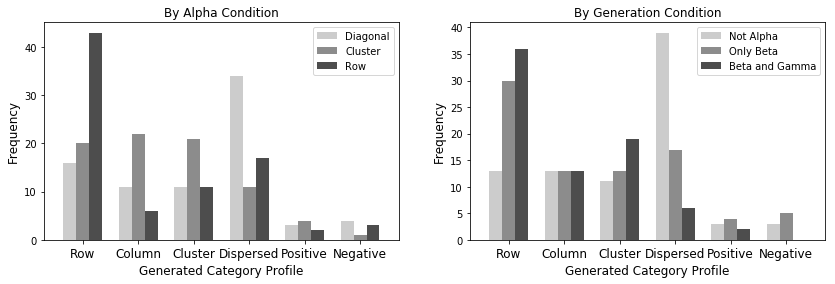
\includegraphics[width=\textwidth]{Figures/profile_freq.png}
\end{center}
\caption{Frequencies of category generation profiles broken down by Alpha condition (left plot) and generation condition (right plot).}
\label{fig:profile}
\end{figure*}

Focusing on the distributional statistics, when broken down by the Alpha conditions (Figure \ref{fig:stats_cond}), we found that the Cluster conditions tended to have categories with a smaller range of both features, and with correspondingly small sizes. The Row conditions produced categories that are high on the x dimension but not the y dimension. These observations indicate that the distributional statistics were carried over from the known category to the generated category in these two Alpha conditions. However, the Diagonal conditions did not have similar distributional statistics observed -- instead of a positive correlation, the Diagonal conditions tended to produce large, dispersed categories. \cite{austerweil2018catgen} also observed a similar effect (although they found more evidence for a negative correlation). Overall, in alignment with previous research, at least two out of the three Alpha conditions in our experiment generated categories that share distributional statistics as the known category.

More interestingly, when the data is broken down by the generation conditions (Figure \ref{fig:stats_instr}), we found that compared to the Not-Alpha conditions, there is moderate evidence showing Beta-Only conditions with a lower y dimension range ($t(162) = 3.00$, $BF_{01} = 0.16$) and moderate to strong evidence that their generated categories are smaller in area ($t(162) = 3.16$, $BF_{01} = 0.10$). There is moderate evidence that the Not-Alpha and Beta conditions share equal range of x dimension values ($t(162) = 1.33$, $BF_{01} = 4.82$). With Beta-and-Gamma conditions, we find greater evidence for smaller and tighter categories compared to the Not-Alpha conditions. Specifically, there is very strong evidence that both Beta and Gamma categories from the Beta-and-Gamma condition are smaller in both x ($t(156) = 4.83$, $BF_{01} = 2.55 \times 10^{-4}$; $t(156) = 4.21$, $BF_{01} = 2.94 \times 10^{-3}$, respectively) and y ($t(156) = 4.57$, $BF_{01} = 7.40 \times 10^{-4}$; $t(156) = 7.56$, $BF_{01} = 4.30 \times 10^{-10}$, respectively) ranges compared to the Not-Alpha conditions. Similarly, there is very strong evidence that both categories in the Beta-and-Gamma conditions are smaller in area than the Not-Alpha conditions ($t(156) = 5.70$, $BF_{01} = 5.41 \times 10^{-6}$; $t(156) = 7.69$, $BF_{01} = 2.07 \times 10^{-10}$, respectively). Overall, when comparing the Not-Alpha conditions to categories from other generation conditions, we consistently find moderate to very strong evidence that Not-Alpha categories are more widely dispersed (in their range values) and also larger (in their area), with the only exception being the comparison of x dimension ranges between the Not-Alpha and Beta-Only conditions.

When comparing the distributions of the Beta and Gamma categories generated within the Beta-and-Gamma conditions, we find an overall weak-to-moderate evidence for equal distributional statistics. Specifically, there was moderate evidence for equal x dimension ranges ($t(150) = 0.56$, $BF_{01} = 9.47$) and weak evidence for both feature correlations and area size ($t(150) = 1.85, BF_{01} = 2.10$; $t(150) = 1.77$, $BF_{01} = 2.40$, respectively). When measured on their y dimension ranges, we found weak evidence for lower values from Gamma categories compared to the Beta categories ($t(150) = 2.47$, $BF_{01} = 0.59$).

% \begin{table}[H]
% \begin{center} 
% \caption{Results of Bayesian $t$-test between the generation conditions: pairwise comparisons of Not-Alpha (A') and Beta-Only (B) conditions, as well as the Beta (BC-B) and Gamma (BC-C) categories separately from the Beta-and-Gamma condition.} 
% \label{table:samplesize} 
% \vskip 0.12in
% \begin{tabular}{llcc} 
% \hline
% Group 1 & Group 2  & $t$(df) & $BF_{01}$ \\
% \hline
% A'   & B    &  3.16(162) & $9.81\times10^{-2}$ \\
% A'   & BC-B &  5.70(156) & $5.41\times10^{-6}$ \\
% A'   & BC-C &  7.69(156) & $2.07\times10^{-10}$ \\
% B    & BC-B &  2.48(156) & $0.58$ \\
% B    & BC-C &  4.27(156) & $2.35\times10^{-3}$ \\
% BC-B & BC-C &  1.77(150) & $2.40$      \\
% \hline
% \end{tabular} 
% \end{center} 
% \end{table}

\begin{figure*}%[H]
\begin{center}
    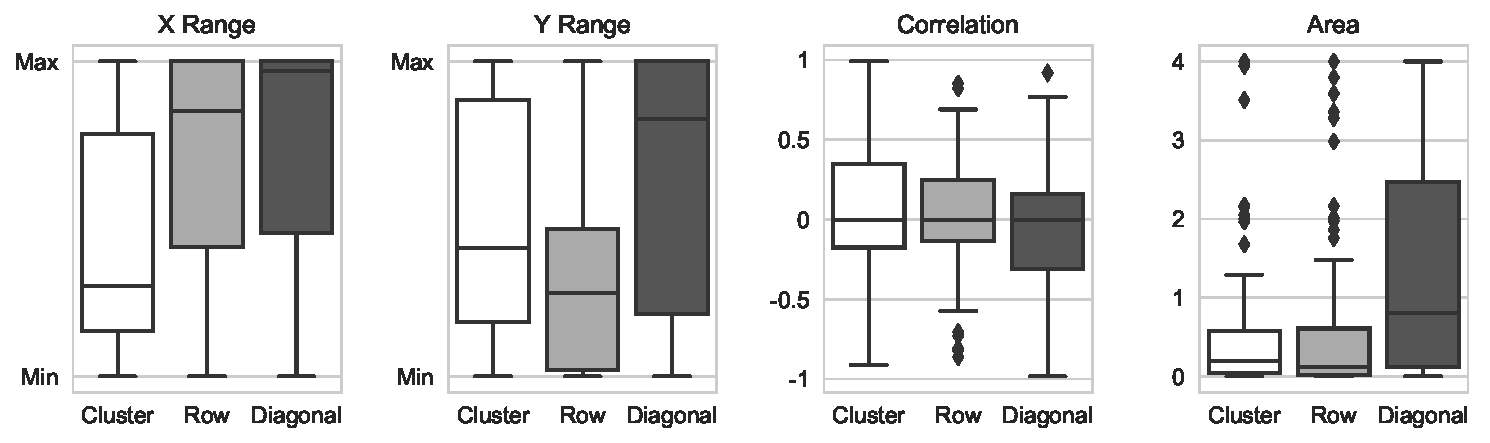
\includegraphics[width=\textwidth]{Figures/stats_cond.pdf}
\end{center}
\caption{Box-plots of the distributional statistics from the generated categories. Boxes depict the median and quartiles of each Alpha condition, with whiskers placed at 1.5 inter-quartile range. All points outside this region are marked individually.} 
\label{fig:stats_cond}
\end{figure*}

\begin{figure*}%[H]
\begin{center}
    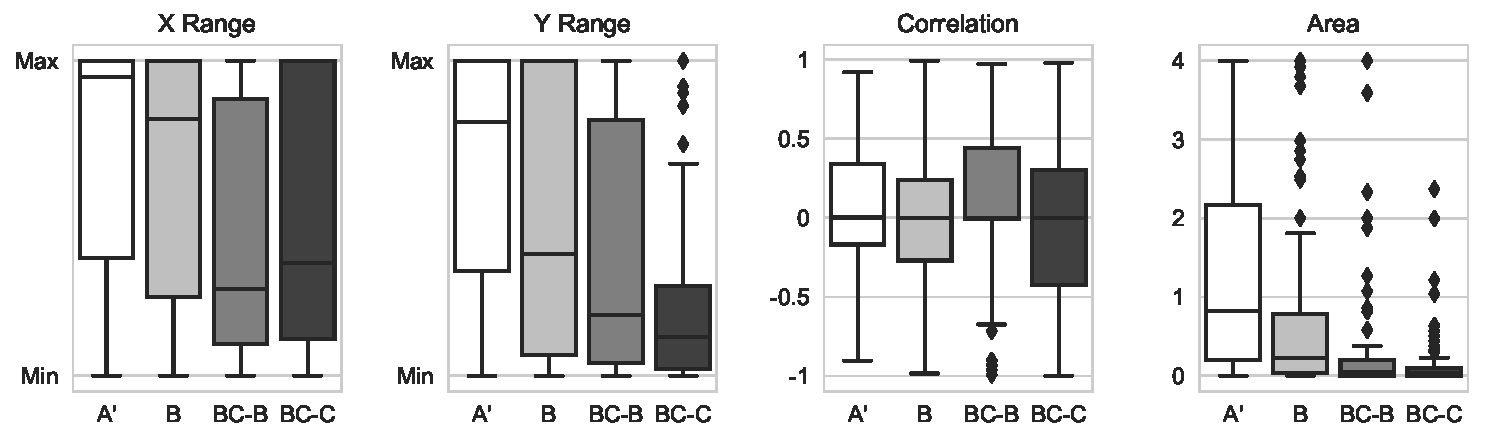
\includegraphics[width=\textwidth]{Figures/stats_instr.pdf}
\end{center}
\caption{Box-plots of the distributional statistics from the generated categories. Boxes depict the median and quartiles of each generation condition, with the Not-A condition denoted by A' and the Beta-Only condition denoted by B. Data from the Beta-and-Gamma conditions are separated into the Beta groups (denoted BC-B) and the Gamma groups (denoted BC-C) generated in that condition. Whiskers are placed at 1.5 inter-quartile range. All points outside this region are marked individually.} 
\label{fig:stats_instr}
\end{figure*}

\section{Discussion}
At first glance, it seems reasonable to assume that generating a new category Y after learning category X is the same as generating a new category Not-X. An independently identified category should already be a category-by-negation (in that an independently identified category is not what was previously known.) Further, if the categories are already identified by arbitrary labels, then it may be easy to assume that identifying the negation of a known category cannot add any additional information in category generation.  

Our results have indicated otherwise. Specifically, when tasked to produce categories-by-negation, participants tended to generate wider and larger new categories compared to when tasked with producing independently identified categories. To our knowledge, this paper represents the first piece of evidence distinguishing these separate types of categories. 

Aside from demonstrating a new effect, this study has continued to show the robustness of the distributional similarities between learned and generated categories. In this sense, the results from the different Alpha conditions are similar to those observed in \cite{austerweil2018catgen}. The generated categories from the Cluster condition tend to possess lower x and y ranges, with a correspondingly smaller area, and the generated categories from the Row condition tend to adopt Row-type profiles. There is also similar lack of categories with positively correlated features from the Diagonal condition.  

However, one notable difference is that while \cite{austerweil2018catgen} found evidence of negatively-correlated
generated categories in their XOR condition, we found no evidence of negatively-correlated generated categories in our
comparable Diagonal condition. \cite{austerweil2018catgen} explained that the presence of negatively-correlated features
in this condition was indicative of the effect of category contrast -- that is, categories with negatively correlated
features are generated because they are particularly different to categories with positively correlated features. It is
possible that due to the reduced strength of the positive correlation in our study compared to
\cite{austerweil2018catgen} (because of the addition of noise to the feature values), participants were no longer as
sensitive to the negative correlations in the experimenter-defined category and therefore started to produce
uncorrelated but widely dispersed categories.

Beyond replicating previous studies, the current study has demonstrated that the consistency in distributional
statistics can persist beyond the first generated category. However, evidence showing this was ultimately weak. One
possible reason for this is the relatively small feature space employed in the tasks. The generation of a second novel
category is necessarily more constrained in the feature space than the generation of the first novel category, possibly
contributing to differences in distributional structure. By exploring stimuli features with less defined boundaries
(e.g., orientation), we may expect to see greater consistency in distributional structure over multiple generated
categories.

Although we have observed participants generating multiple independently identified categories, we do not want to imply that categories-by-negation can only happen once. It would be worth investigating how participants might proceed to generate additional categories-by-negation (e.g., by asking observers to generate a category that is Not-Alpha and Not Beta). Packing Theory \citep{hidaka2011packing} -- a hypothesis that suggests categories can be neatly `packed' into the feature space -- may indicate that successive categories-by-negation are generated in a fashion that preferentially occupies spaces between observed categories. Further, although none of the current models of category generation can directly account for the effects observed in this study, they may be useful components in a larger category generation framework. For instance, future work may consider implementing the hierarchical sampling model from \cite{jern2013probabilistic} in a framework of overhypotheses \citep{kemp07}, where a prior can be placed over a category identity space, allowing models to behave differently under different regions of generated category identity.

Ultimately, the nature of newly generated categories appears to vary depending on the identity they were associated
with. The extent to which they may differ, and the mechanisms driving these differences represent fascinating areas for
future research.

\section{Acknowledgments}
This work was funded by a Vilas Life Cycle Professorship and the VCRGE at University of Wisconsin-Madison with funding from the WARF


% In the \textbf{initial submission}, please \textbf{do not include
%   acknowledgements}, to preserve anonymity.  In the \textbf{final submission},
% place acknowledgments (including funding information) in a section \textbf{at
% the end of the paper}.

\bibliographystyle{apacite}

\setlength{\bibleftmargin}{.125in}
\setlength{\bibindent}{-\bibleftmargin}

\bibliography{citations.bib}


\end{document}
